\documentclass{article}
\usepackage{graphicx}
\usepackage{hyperref}
\usepackage{listings}
\usepackage{amsmath}
\usepackage{amssymb}
\usepackage{geometry}

\newgeometry{vmargin={20mm}, hmargin={20mm,20mm}}
\title{\textbf{COP290 C Lab} \\ Terminal Based Spreadsheet Application}
\date{\vspace{-5ex}}
\author{Lucky Ahirwar \\
        2022CS52049 \\
        \and Swapnil \\
        2022ME21540 \\
        \and Panugothu Saicharan \\
        2023CS10080 }
        
\begin{document}

\maketitle
\iffalse
\begin{abstract}
This report describes the development of a terminal-based spreadsheet application. It provides an overview of the project's features, design choices, data structures used, and the integration of various components. The report also details the challenges faced and the overall architecture of the application.
\end{abstract}
\fi

\section{Introduction}
Spreadsheets are widely used for data organization, computation, and analysis. This project implements a spreadsheet application that operates entirely within a terminal. The goal was to create an efficient and lightweight solution with fundamental spreadsheet functionalities, including data storage, arithmetic operations, and formula evaluation.

\section{Features}
The terminal-based spreadsheet application provides the following functionalities:
\begin{itemize}
    \item Quick and efiicient data storage and retrieval.
    \item Basic arithmetic operations such as addition, subtraction, multiplication, and division.
    \item Support for cell references in formulas (e.g., A1 + B2).
    \item Support for range functions MIN, MAX, SUM, STDEV, AVG.
\end{itemize}

\section{High-Level Design}
The application follows a modular design, with key components including:
\begin{itemize}
    \item \textbf{Parser and Evaluator}: Parses user inputs, identifies commands and errors, and sends response to Evaluator. Evaluator checks for further errors, like presense of cycles, division by zero, and then adds data to cells, updates dependecies, and reevaluates the values of cell affected by the changes.
    \item \textbf{Data Storage Module}: Manages the spreadsheet grid using an array of pointers to deque-like structure. Each column is represented by this struct. Initially all pointers are NULL. But as we add items to rows, the deque is filled. Each deque segment stores values for a range of rows (e.g., from 0 to 99, from 200 to 299, from 100 to 199).
    \item \textbf{User Interface}: Handles command-line interactions and rendering of the spreadsheet. Gets the input and displays the time spent on the computation, and if there is an error, displays the error message.
\end{itemize}

\begin{figure}[ht]
    \centering
    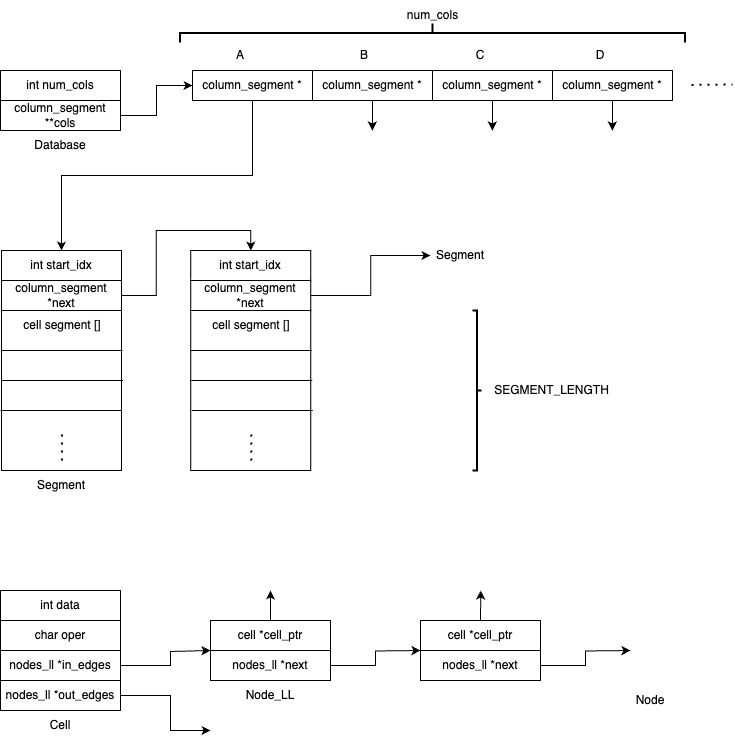
\includegraphics[width=0.5\textwidth]{docs/hld.png}
    \caption{High-Level Design of the Database}
    \label{fig:high_level_design}
\end{figure}

\section{Data Structures Used}
To ensure efficient performance, the following data structures were utilized:
\begin{itemize}
    \item \textbf{Linked List}: Used to manage edges in the dependency graph.
    \item \textbf{Graph (Dependency Graph)}: Tracks dependencies between cells for formula calculations.
    \item \textbf{Deque}: Implements efficient column-wise storage of cell data.
\end{itemize}

\section{Component Breakdown}
\subsection{Data Storage}
Each cell is represented using a struct that contains its value, an operator, an error flag, and pointers for dependency tracking.

\subsection{Parser and Evaluator}
The parser processes user inputs, distinguishes between direct values and expressions, and forwards expressions to the evaluator. The evaluator computes values while maintaining dependency tracking. The evaluation module includes built-in functions such as sum, average, and standard deviation.

\subsection{User Interface}
A command-line interface (CLI) is implemented to provide an intuitive interaction mechanism. Commands allow users to modify cells, apply formulas, and navigate through the spreadsheet.

\subsection{Dependency Graph}
A linked list-based graph tracks dependencies between cells, ensuring correct recalculations when referenced cells change.

\section{Integration and Workflow}
When a user inputs a command, the following steps occur:
\begin{enumerate}
    \item The input is passed to the parser, which categorizes it.
    \item If it is a formula, dependencies are analyzed using a graph structure.
    \item The evaluator computes the value if necessary and updates the data storage.
    \item The UI updates the display to reflect changes.
\end{enumerate}

\iffalse
\section{Challenges and Optimizations}
Some of the challenges encountered include:
\begin{itemize}
    \item Efficiently handling formula dependencies and cyclic references.
    \item Managing memory usage for large spreadsheets.
    \item Optimizing parsing and evaluation speed.
\end{itemize}
Optimizations include:
\begin{itemize}
    \item Using a graph-based approach to track dependencies and avoid redundant calculations.
    \item Implementing lazy evaluation for improved performance.
    \item Utilizing hash sets for quick access to stored cell data.
\end{itemize}
\fi

\section{Conclusion}
This project successfully implements a functional spreadsheet application for terminal users. With its modular architecture, efficient data handling, and core spreadsheet functionalities, it provides a lightweight alternative to traditional GUI-based spreadsheets. Future enhancements may include advanced functions, improved UI, and multi-user collaboration features.

\end{document}
